\ifbook{

}

\ifslide{
 \section{Brief reminder - multiple choice}

 % TODO

  \section{Agenda}
  \begin{frame}{Agenda}
    \begin{block}{Session outline}
      \begin{itemize}
        \item Hello World
        \item Java syntax and purpose of a syntax
        \item Identifier
        \item Comments
        \item Core data types
        \item Operators
        \item Strings
      \end{itemize}
    \end{block}
  \end{frame}

  \section{The Hello World}

  \begin{frame}{First program in Java}
    \begin{block}{Instructions}
      \begin{itemize}
        \item Download the HelloWorld.java file and save it on the Desktop
        \item Start a \textbf{Terminal} in the application menu
        \item Change the current directory of the terminal by using the following command:
        \begin{itemize}
          \item \texttt{pwd} - prints current directory
          \item \texttt{ls} - displays the files of the directory
          \item \texttt{cd <directory>} - change to directory provided as arguments
          \item \texttt{man <command>} - help for the command
        \end{itemize}
        \item Once the current directory of the Terminal is Desktop, compile the file:
        \begin{itemize}
          \item \texttt{\$ javac HelloWorld.java}
        \end{itemize}
        \item Once the code has compiled, execute it:
        \begin{itemize}
          \item \texttt{\$ java HelloWorld}
        \end{itemize}
      \end{itemize}
    \end{block}
  \end{frame}

  \begin{frame}{Results}
   \begin{center}
     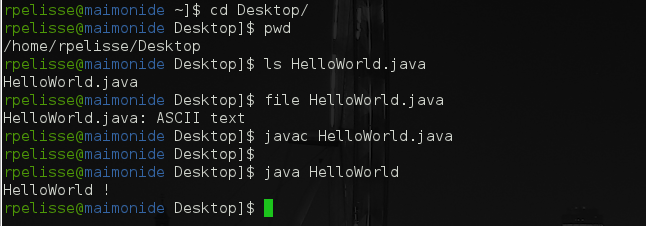
\includegraphics[scale=0.5]{img/hello-world.png}
   \end{center}
  \end{frame}

  \begin{frame}{Communicating with the program}
    \begin{block}{Arguments}
      \begin{itemize}
        \item Download the Arguments.java file and save it on the Desktop
        \item Compile and execute the program, adding some arguments:
        \item \texttt{\$ java Argument The answer is 42.}
      \end{itemize}
    \end{block}
    \begin{center}
      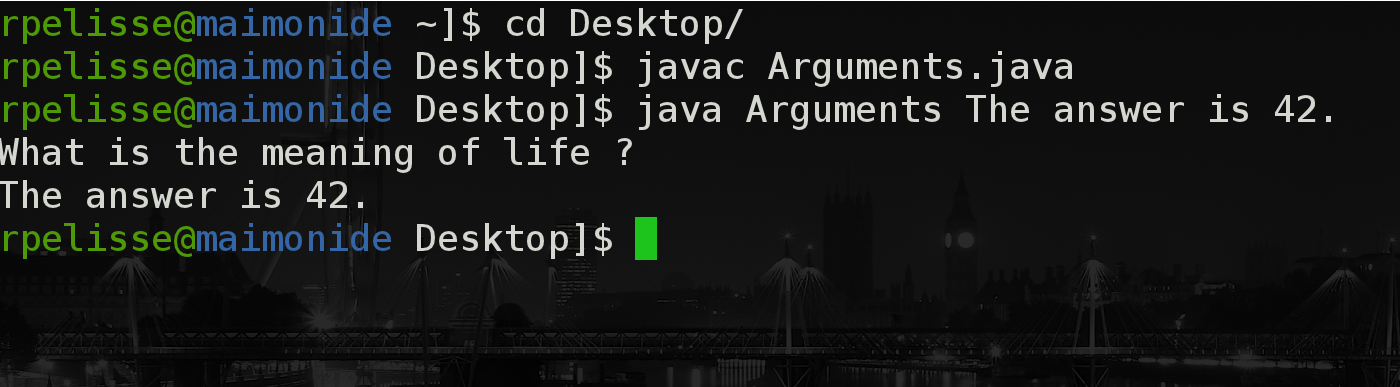
\includegraphics[scale=0.2]{img/arguments.png}
    \end{center}
  \end{frame}

  \section{Java and its syntax}
  \subsection{File organization}
  \begin{frame}
    \begin{block}{What does a source file contains ?}
      \begin{itemize}
        \item look at the HelloWorld class and identify the different section:
        \begin{itemize}
          \item header
          \item comment
          \item class name
        \end{itemize}
      \end{itemize}
    \end{block}
    \begin{center}
      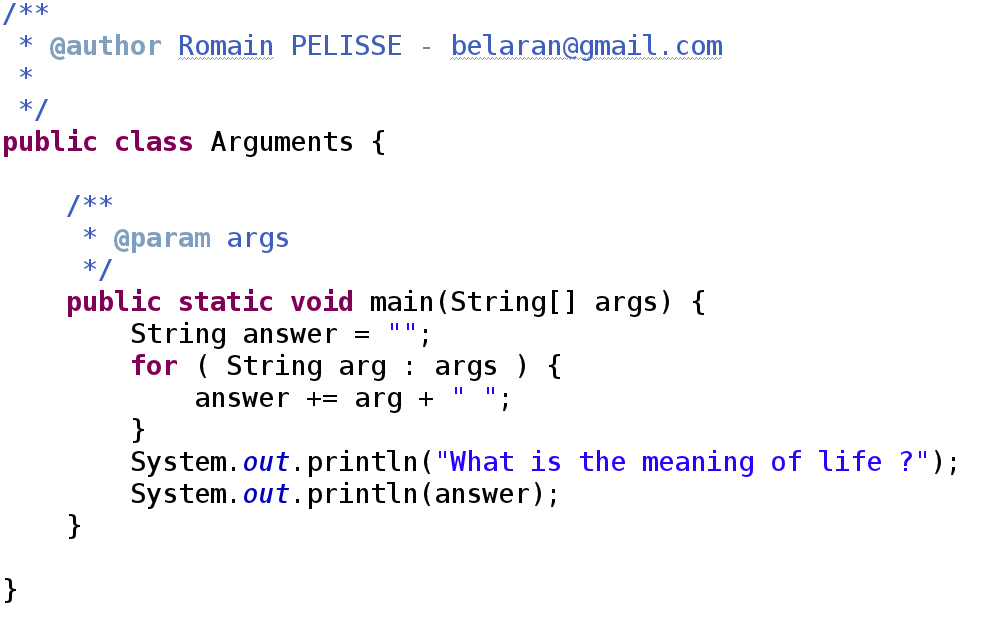
\includegraphics[scale=0.2]{img/java-source-file.png}
    \end{center}
  \end{frame}
  \subsection{Variables}
  \begin{frame}
    \begin{block}{Variable - how to store and manipulate data}
      \begin{itemize}
        \item What is a variable ?
        \begin{itemize}
          \item memory allocation to store date
          \item the data is \textbf{typed}
        \end{itemize}
        \item What can do with them ?
        \begin{itemize}
          \item change the value
          \item use operator
        \end{itemize}
      \end{itemize}
    \end{block}
    \begin{center}
      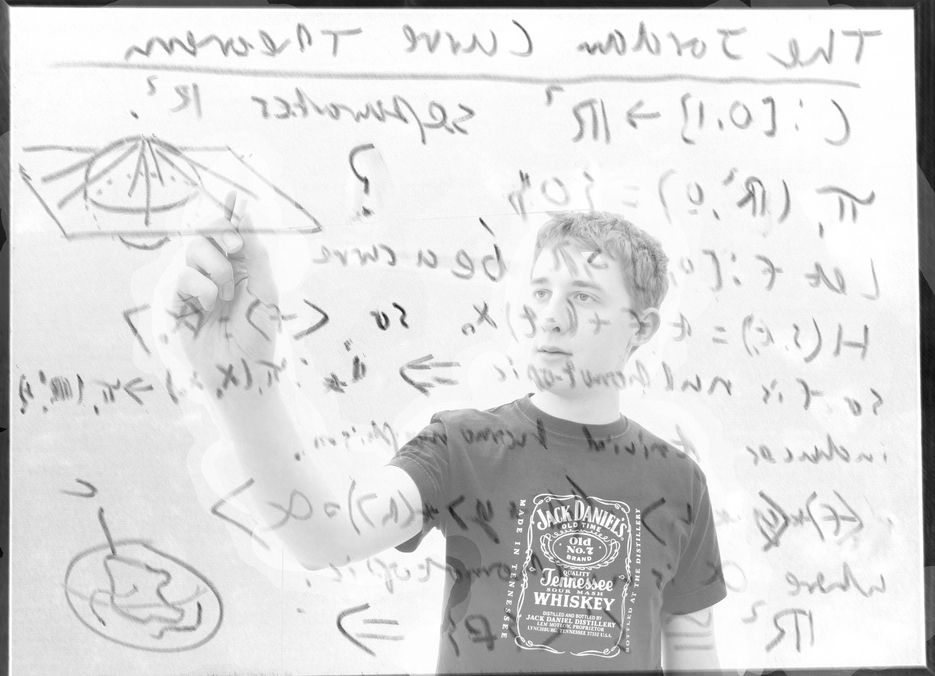
\includegraphics[scale=0.2]{img/variables.jpg}
    \end{center}
  \end{frame}

  \begin{frame}
    \begin{block}{Java primitives}
      % what the point of short, double if we generally use int ?
      % what are the "risk" or advantages of using short or long ?
      % why use boolean over an int with 0,1 ?
      \begin{description}
        \item[byte] an 8-bit signed integer - value range: -128 to 127 (inclusive)
        \item[short] a 16-bit signed  integer - value range:-32,768 to 32,767 (inclusive)
        \item[int] a 32-bit signed - value range: -2,147,483,648 to 2,147,483,647 (inclusive)
        \item[long] a 64-bit signed - value range: -9,223,372,036,854,775,808 to 9,223,372,036,854,775,807 (inclusive)
        \item[float] a single-precision 32-bit IEEE 754 floating point.
        \item[double] a double-precision 64-bit IEEE 754 floating point
        \item[boolean] has only two possible values: true and false
        \item[char] a single 16-bit Unicode character
      \end{description}
    \end{block}
  \end{frame}
  \subsection{Operator}
  \begin{frame}
    \begin{block}{Playing with variables - Operator}
      \begin{itemize}
        \item Download the Addition.java file and save it on the Desktop
        \item Compile it and execute it:
        \begin{itemize}
          \item \texttt{\$ java Addition 1 2}
        \end{itemize}
        \item Exercices:
        \begin{itemize}
          \item copy this file and rename it \textbf{Substract.java} - change this new file to
          implement a substraction
          \item in \textbf{Addition.java}, replace the \texttt{int} by \texttt{short} and run the
          program with inputs 5 and 128. What is happening ? Why ?
          \item do we really need \textbf{variables} for this program ? How can we do
          \textbf{without} using variables ?
          \item adapt \textbf{Addition.java} in order to have the program able to do addition with
          \textbf{money}
        \end{itemize}
      \end{itemize}
    \end{block}
  \end{frame}

  % Introducing the "useless" data type => character

  % Function calls

}
